\begin{abstract}
  The aim of the report is to briefly introduce the concept of
  data-parallel paradigm and to study and evaluate the implementation of
  a stencil skeleton, a particular parallel computation in which data
  dependence pattern is implemented by the mean of inter-worker
  communications.
\end{abstract}

\section{Introduction}

A data parallel computation, which can be defined both on streams and or
single data value, consists in the partition of possibly large data
structures to different processing entities which are able to compute
a function on the assigned partition in parallel. This parallel pattern
bases its functionalities on function replication. As a consequence, the
knowledge of the sequential computation form is necessary both for
function replication and data partitioning. This is the main reason for
the parallel program design complexity. Latency and memory capacity are
optimized compared to other stream parallel paradigms like farms, though
a potential load unbalance exists.

\begin{wrapfigure}{r}{0.25\textwidth}
  \centering
  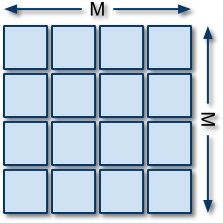
\includegraphics[width=0.2\textwidth]{imgs/stencil.png}
  \caption{Data parallel partition scheme}
  \label{fig:data-parallel}
\end{wrapfigure}


To better understand, let us consider a data parallel computation
operating on a bi-dimensional matrix as depicted in
Figure~\ref{fig:data-parallel}. The matrix is partitioned in blocks of
$g = {M^{2} \over n}$ elements. Successively each block is transmitted
to each worker through a \emph{scatter} operation. Then all workers
apply the same function $F$ to the corresponding partition in parallel.
At the end, the result may be collected through a \emph{gather}
operation.


\begin{description}
  \item[Map]\hfill\\
    {When all the workers are \emph{fully independent} and
    operate on their own partition, without any cooperation}
  \item[Stencil-based]\hfill\\
    {When a workers operate in parallel and
    \emph{cooperate} through data exchanges. In this case data
    dependencies are implemented by inter-worker communications.}
\end{description}

The form of a stencil may be \emph{statically} predictable or
\emph{dynamically} exploited according to the current data values. In
case of static stencil we have two other possibilities: a \emph{fixed}
stencil where the communication scheme is fixed throughout the
computation, and a \emph{variable} stencil where the communication
scheme varies from a computation step to the next one, although the
overall behavior is statically predictable.

In this report we will concentrate our attention to \emph{static fixed
stencils} applied on bi-dimensional matrix.

\section{Abstract implementation}\label{sec:abstract-impl}

In this section we briefly discuss the general idea of our
implementation leaving the implementation details out of this section.
The interested reader can find a more detailed analysis of the real
implementation in ``\nameref{sec:concrete-impl}'' section.

The main idea we followed is very simple. Since we are dealing with a
data-parallel pattern, some kind of partition of the input problem is
required to properly solve the problem. The schema can be synthesized in
four steps:

\begin{enumerate}
  \item The input matrix is loaded by the collector and equally split
    among the available workers
  \item Each worker communicate its contour segments needed to the other
    neighbors
  \item After having received the necessary data from the neighbors, the
    computation on the given partition is started in parallel on each
    worker
  \item The resulting partition is sent back toward a collector, which
    is in charge of collating partial results, thus providing the final
    result.
\end{enumerate}

As you might imagine, the central point in this scheme which can
introduce substantial optimization is the partition phase. This can be
implemented in different ways on the basis on the input offsets.

\begin{figure}[!h]
  \subfigure[Partition by row]{
    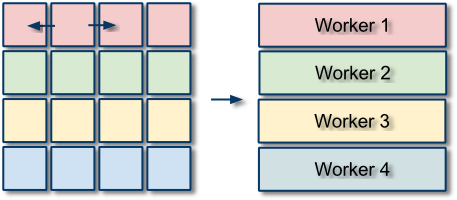
\includegraphics[width=0.3\textwidth]{imgs/row-part.png}
  }
  \hfill
  \subfigure[Partition by column]{
    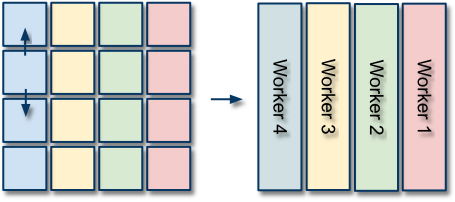
\includegraphics[width=0.3\textwidth]{imgs/col-part.png}
  }
  \hfill
  \subfigure[Partition by blocks]{
    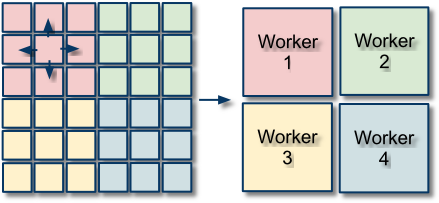
\includegraphics[width=0.3\textwidth]{imgs/block-part.png}
    \label{fig:part-scheme-block}
  }
  \caption{Different partition schemes}
  \label{fig:part-scheme}
\end{figure}


In our implementation, the partition phase tries to derive an optimal
partition by trying to minimize the communication between workers. We
have isolated three different situations depicted, which are depicted in
Figure~\ref{fig:part-scheme}:

\begin{description}
  \item[Row partition] Whenever the input offsets set contains
    dependencies that are row dependent only, a row partition scheme is
    derived. This means that all the elements in the input offset set
    are of the type \emph{(0,$x$)}. In this case no communication at
    all is required between workers, therefore a full \emph{map}
    parallelism is possible if each worker has an entire row
    assigned.

  \item[Column partition] This is the mirror of the \emph{row partition}
    case and it is verified whenever a given element depends only on
    elements which are on the same column. In this situation the input
    offset set contains only elements of the type \emph{($x$, 0)}. No
    communications is required, on the condition that at each worker is
    assigned an entire column of the input matrix.

  \item[Block partition] Whenever a \emph{row} neither a \emph{column
    partition} is applicable, a block partition is derived. In this case
    the input offset set contains ``heterogeneous'' points, so no kind
    of trivial derivation is possible. In our case a minimum rectangle
    called ``Elementary Rectangle'' is derived. This rectangle is
    evaluated by taking as reference point a single element and deriving
    the smallest rectangle that encompass all data dependencies needed to
    evaluate the function in that specific point.
\end{description}

If we are in presence of a \emph{Block partition} situation another
optimization is still possible. Indeed, we can try to still partition
the matrix by ``row-blocks'' or ``column-blocks'' by vertically or
horizontally stacking single \emph{elementary rectangles} thus achieving
a more optimized partition. In fact this situation is able to avoid
communications between ``elementary'' workers that are still present in
a situation like the one depicted in Figure~\ref{fig:part-scheme-block}.

\section{Cost model: completion time}

Since the cost model specifically depends on the offsets passed as input
to the stencil skeleton, we have decided to derive a general
approximated cost model which tries to collect the most configurations
still maintaining a reasonable precision in the evaluation. Before
reaching the final formulation, we explain the steps the brought us to
the successful derivation.

In our case the starting matrix is read from the disk and then
partitioned in some way among $n$ workers through the use of a remote
communication which has a cost of $T_{scatter}(n,g)$, where $g$ is the
block size assigned to each worker ($g = {M^{2}\over n}$, assuming
``balanced'' partitions).

Then each worker after having received its own partition, is in charge
to communicate to all the neighbors the necessary contour partition. Of
course, this communication has an associated cost, which has to be
evaluated but varies according to the specific input offsets passed to
the skeleton. To model this part of the formula we have to introduce a
parameter which is $rc$ (real communications), which represents the
number of communications we have to make with the neighbors. To better
understand the situation, let's assume to have as input offsets:
\emph{(0, -1), (-1, 0), (0, 1) (1, 0)}

\begin{figure}[!h]
  \centering
  \subfigure[Elementary partition]{
    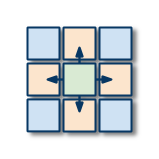
\includegraphics[width=0.2\textwidth]{imgs/part-elem.png}
    \label{fig:part-elem}
  }
  \quad
  \subfigure[Partition by row]{
    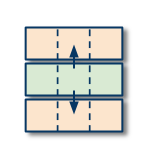
\includegraphics[width=0.2\textwidth]{imgs/part-row.png}
    \label{fig:part-row}
  }
  \caption{Two ways of partitioning the same matrix}
  \label{fig:part-overview}
\end{figure}

The situation is the one depicted in Figure~\ref{fig:part-elem}. In this
case we are assuming the ``elementary'' partition 1 by 1 where each
worker has responsibility for just 1 matrix element. In this case before
starting the computation the worker has to communicate respectively to
the upper, next, lower and previous neighbor its data partition,
assuming the “owners-compute-rule” to be satisfied. At the end the
parameter $rc$ will be 4. This has to be multiplied by the $T_{comm}(P)$
where P represent the size of the data to be transmitted to the
neighbors. In this specific case this is equal to 1, but in other cases
this may vary based on the size of the partition and the offsets, as you
will see. In fact, by keeping the same input offsets and by only
changing the size of the sub-matrix partition assigned to each worker
the things changes, as presented in Figure~\ref{fig:part-row}. In this
specific case, not only the P parameter changes and becomes 3 but also
the $rc$ changes to 2.

Then a calculation phase is started in parallel by each worker on its
specific partition which takes a total time of $g \cdot T_{f}$, where
$T_{f}$ is the time needed to calculate the function among all inputs
(in our case 5 considering the central value) while $g$ is the size of the
partition assigned to each worker or better the number of items a given
worker has assigned inside the partition.

At the end of the calculation, a second phase is started which consists
in transferring back the computed partition to the root node
($T_{gather}(n,g)$). This can be evaluated by simply taking into account
the double communication at the first phase. Thus the resulting formula
is:

$$
2 T_{scatter}(n,g) + rc \cdot T_{comm}(P) + g \cdot T_{f}
$$

As a measure of comparison, the sequential algorithm cost model is given
by the last part of the previous formulation, considering that the
partition in this case is the entire input matrix: $M^{2} \cdot T_{f}$.

\section{Performance measurements and tests}

% TODO: possiamo aggiungere il fatto della derivata e che abbiamo
% utilizzato solo 8 nodi perche ci sono gli utenti idioti che spengono
% il pc :)

In this section we present performance measurements we have collected
during our experiments. For this scope we have decided to test two
different functions with different complexity. The first one is
\texttt{min} which applied to various elements returns the minimum among
them. The latter is \texttt{linsolve} a simple function which tries to
solve a system of linear algebra equations. The only assumption we made
during the experiment was to have as input offsets the following set:
\emph{(0, -1), (-1, 0), (0, 1) (1, 0)}.

To better understand the final goal of the \texttt{linsolve} function
take in consideration the scheme below, which assumes ``\emph{e}'' as
the target element to be computed:

\[
\left(
\begin{array}{ccc}
  a & b & c \\
  d & e & f \\
  g & h & i
\end{array}
\right)\rightarrow\begin{cases}
  bx + hy = e \\
  dx + fy = e
\end{cases}\rightarrow{result = {{x + y}\over2}}
\]

Regarding the ideal statistics we have used some instrumentation inside
the code to evaluate the calculation time $T_{calc} = M^{2} \cdot T_f$
and used it to derive the correct $T_f$ value.  Results collected and
derived are presented in Table~\ref{tbl:timings}.

\begin{table}
  \centering
  \begin{tabular}{|c|c|c|c|}
    \hline
    \textbf{Function} & \textbf{$M$} & \textbf{$T_{calc}$} (sec) & \textbf{$T_f$} (sec) \\
    \hline
    \texttt{min}      & 3000         & 61.923              & 6.880\e{-06} \\
                      & 4000         & 95.880              & 5.992\e{-06} \\
                      & 5000         & 146.599             & 5.864\e{-06} \\
                      & 6000         & 206.726             & 5.742\e{-06} \\
    \hline
    \texttt{linsolve} & 3000         & 711.255             & 7.903\e{-05} \\
                      & 4000         & 1274.833            & 7.968\e{-05} \\
    \hline
  \end{tabular}
  \caption{Calculation time timings}
  \label{tbl:timings}
\end{table}

Since the implementation we have provided makes use of MPI message passing
library which does not guarantee any constant behaviour for the setup
``socket'' procedure, we preferred to avoid to take in consideration the
$T_{setup}$ parameter which should be paid once for every communication
as $T_{comm}(L) = T_{setup} + L \cdot T_{transm}$ formula suggests. By
the way this is not a wrong assumption, because in MPI after the setup
procedure all peers involved in the MPI ``world'' are free to
communicate each other without paying any more the setup procedure. So
the setup is made once and for all, thus ignoring this parameter, by
placing instrumentation code in proper position, does not impact in any
way our study case.

The evaluation of $T_{transm}$ parameter was simply evaluated by taking
a statistic mean on top of the scattering time of the matrix registered
by our instrumentation code. The resulting value results to be equal to
$3.437\e{-07} {item \over sec}$.

After having set up all the parameters we collected all the needed
timings to derive the proper statistics. Since we were dealing with
a data-parallel skeleton, we have focused our attention on the following
parameters:\\

\begin{tabular}{r | p{0.5\textwidth}| c}
  \textbf{Completion time} & Time needed to complete the computation on
  the given input & $T_c$ \\

  \textbf{Efficiency}      & Provides a measure of how close is the
  effective performance with respect to the ideal one. & $
  \epsilon(n) = {T_{c-id}^{(n)} \over T_{c}^{(n)}}$ \\

  \textbf{Speedup}         & Provides a measure of the relative speed of
  the parallel computation with respect to the sequential one. & $ s(n) =
  {T_{c-id}^{(1)} \over T_{c}^{(n)}} = \epsilon(n) \cdot n$ \\

  \textbf{Scalability}     & The ratio between parallel execution time
  with parallelism degree equal t 1 and the parallel execution with
  parallelism degree equal to $n$ & $scalab(n) = {T_{c}^{(1)} \over
  T_{c}^{(n)}}$
\end{tabular}

\subsection{Statistics for min function}

In this section we present the statistics we have collected regarding
the \texttt{min} function. Since no interesting differences were
reported for the mid-sized cases, we decided to just attach the
statistics regarding the limiting cases. The former when the array size
is equal to 3000 by 3000 elements. The latter where the array is
composed of 6000 by 6000 elements.

A compare between completion time of the two limit cases is presented in
Figure~\ref{fig:min-tc}. As you can imagine, in this situation a solution
of this kind does not offer any kind of advantages, since the time taken
by the function to compute a given element is very low compared to the
effort taken by the skeleton to distribute data and work among workers
through the network. Therefore the transmission overhead highly impacts
on the possibility to scale up.

\begin{figure}[!h]
  \subfigure{
    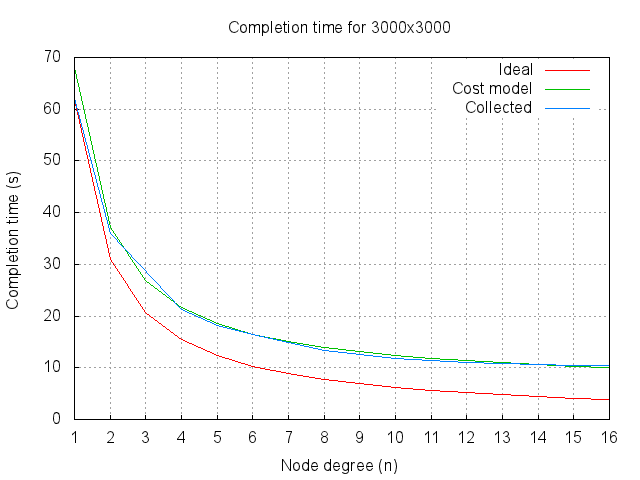
\includegraphics[width=0.45\textwidth]{plots/min/tc-3000.png}
  }
  \subfigure{
    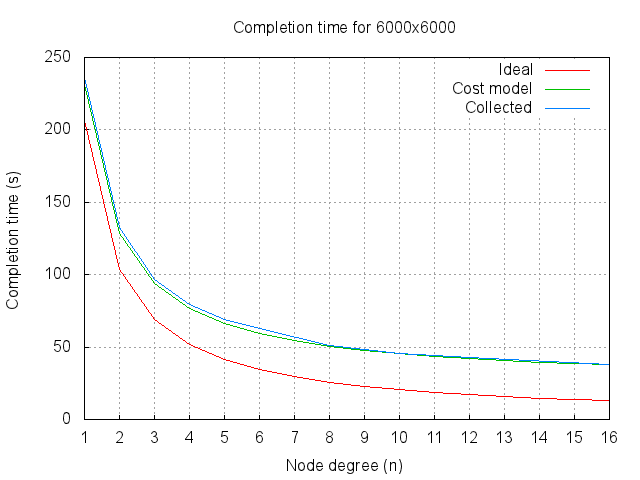
\includegraphics[width=0.45\textwidth]{plots/min/tc-6000.png}
  }
  \caption{\texttt{min} function: Completion time}
  \label{fig:min-tc}
\end{figure}

The thing is more evident if you take as reference
Figure~\ref{fig:min-scal-eff} which presents statistics regarding
speedup, efficiency and scalability. As you can see, for the first case, with the
maximum number of processing elements we can achieve a speedup
equals to 6, which is quite low for the employed resources. By taking in
consideration the second case, an efficiency of less than 35\% produces
a speedup of $\approx 5.5$ for 16 processing elements.

\begin{figure}[!h]
  \subfigure{
    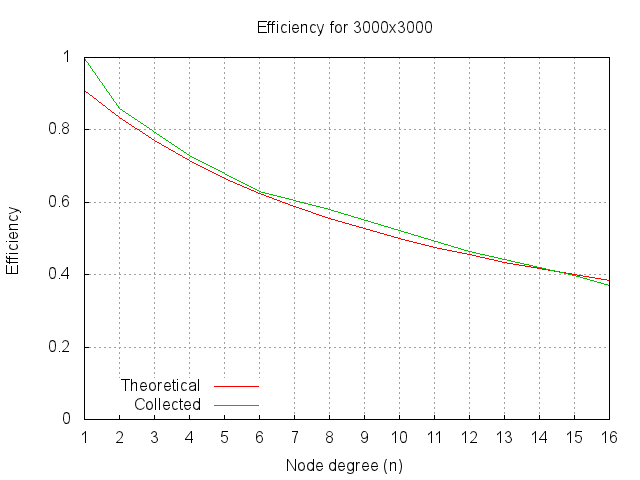
\includegraphics[width=0.45\textwidth]{plots/min/eff-3000.png}
  }
  \subfigure{
    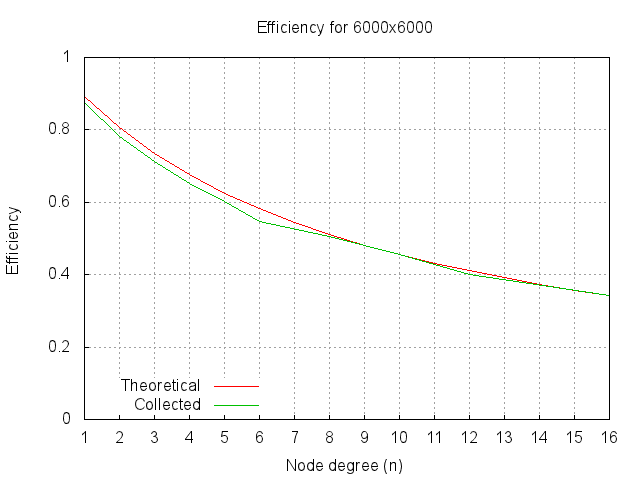
\includegraphics[width=0.45\textwidth]{plots/min/eff-6000.png}
  }\\
  \subfigure{
    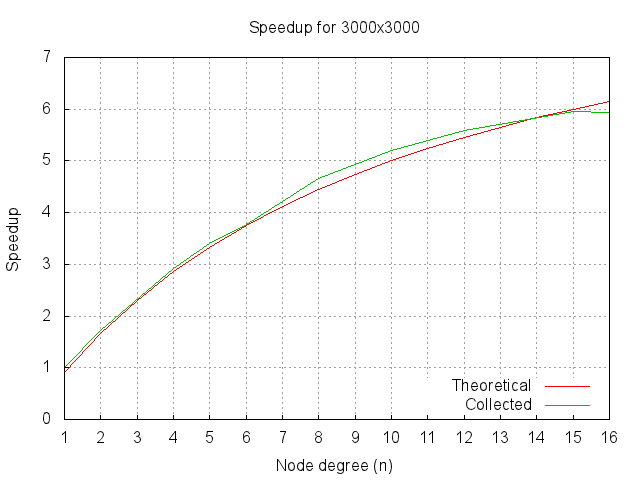
\includegraphics[width=0.45\textwidth]{plots/min/speed-3000.png}
  }
  \subfigure{
    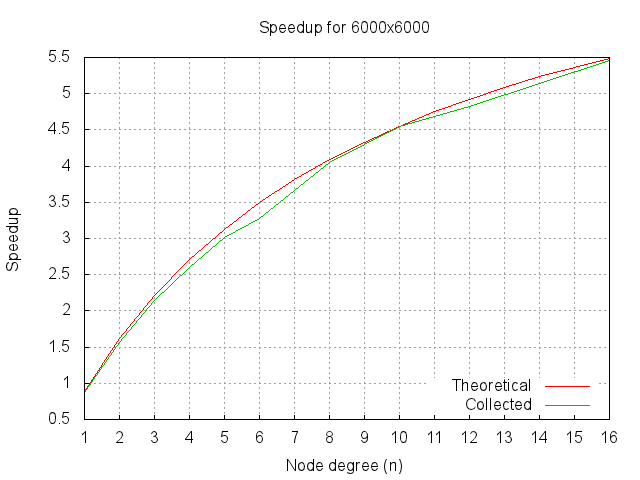
\includegraphics[width=0.45\textwidth]{plots/min/speed-6000.png}
  }\\
  \subfigure{
    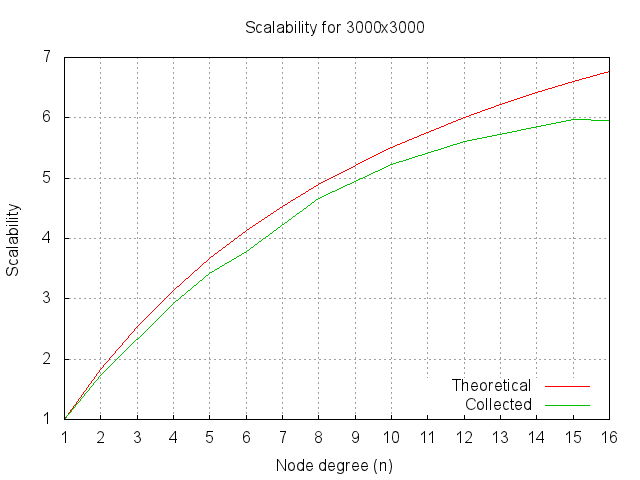
\includegraphics[width=0.45\textwidth]{plots/min/scal-3000.png}
  }
  \subfigure{
    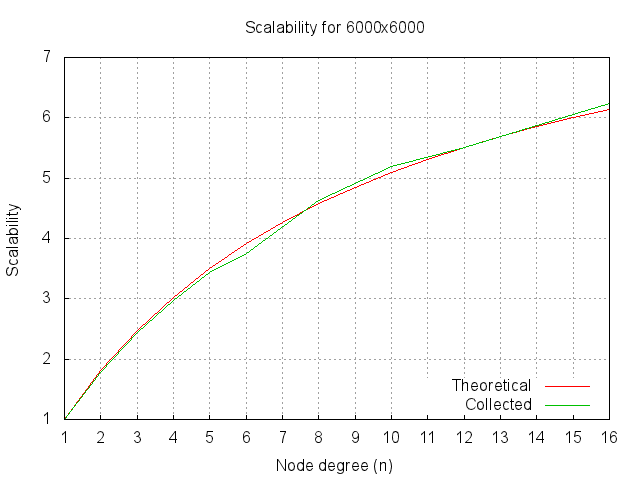
\includegraphics[width=0.45\textwidth]{plots/min/scal-6000.png}
  }
  \caption{\texttt{min} function: Efficiency, Speedup and Scalability}
  \label{fig:min-scal-eff}
\end{figure}

\subsection{Statistics for linsolve function}

Regarding the parallelization of \texttt{linsolve} function, we got
interesting results which demonstrate the goodness of our
implementation. Figure~\ref{fig:linsolve-tc} shows the completion time
graph for the two runs. As you can see, the cost model elaborated really
resemble in a very precise way the behaviour of the program. Indeed all
the three lines almost describe the same decay function. This is because
our computation is time is very large compared to the other overhead we
incur on when we split the matrix through the network of multi-cores.

\begin{figure}[!h]
  \subfigure{
    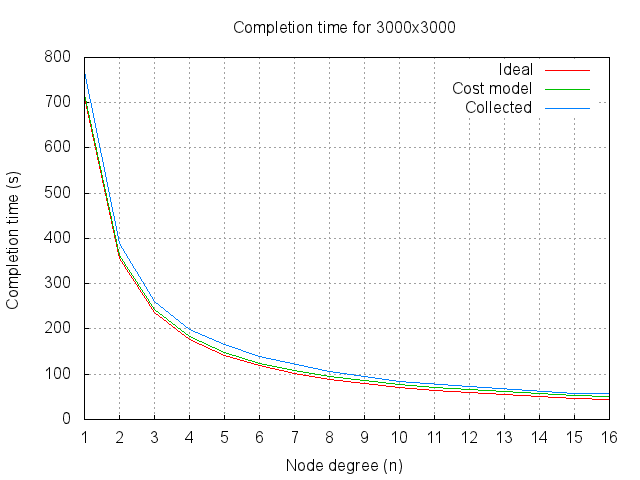
\includegraphics[width=0.45\textwidth]{plots/linsolve/tc-3000.png}
  }
  \subfigure{
    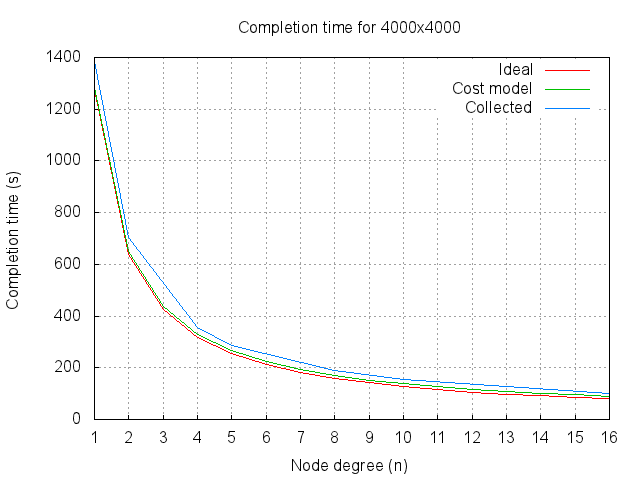
\includegraphics[width=0.45\textwidth]{plots/linsolve/tc-4000.png}
  }
  \caption{\texttt{linsolve} function: Completion time}
  \label{fig:linsolve-tc}
\end{figure}

On the other hand, Figure~\ref{fig:linsolve-scal-eff} shows a comparison
between \emph{speedup} and \emph{efficiency} statistics. As you may
notice, there is the presence of differences between the real and the
predicted situation. Indeed this is not strange at all. The behavior is
mostly caused by the semantic of \texttt{linsolve} function itself. In
fact, the function tends to generate load unbalancing among workers,
thus resulting in a slight increase of completion time and therefore in
fluctuations between theoretical efficiency and the real one. This is
because some partitions might have a major number of solvable systems
while the others might have less or at least simpler one. Anyhow, the
final results demonstrate how much the parameter $T_f$ impacts on the
speedup.

\begin{figure}[!h]
  \subfigure{
    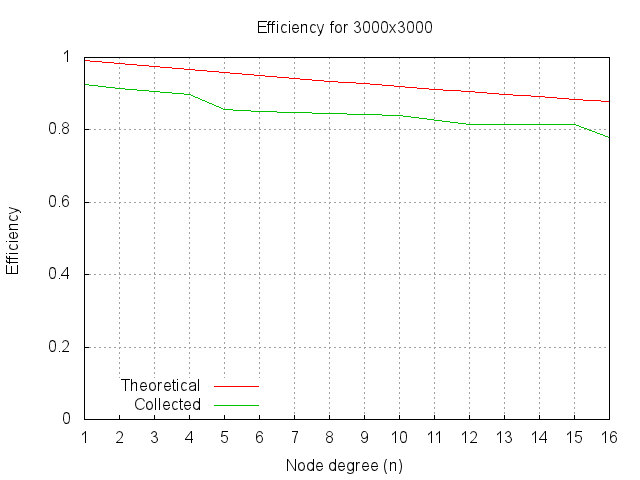
\includegraphics[width=0.45\textwidth]{plots/linsolve/eff-3000.png}
  }
  \subfigure{
    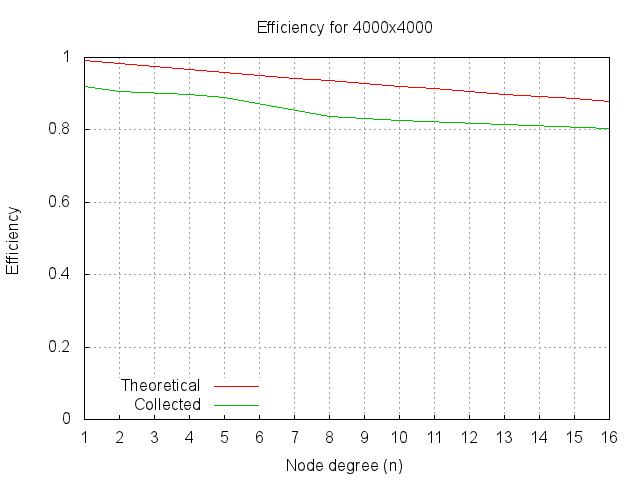
\includegraphics[width=0.45\textwidth]{plots/linsolve/eff-4000.png}
  }\\
  \subfigure{
    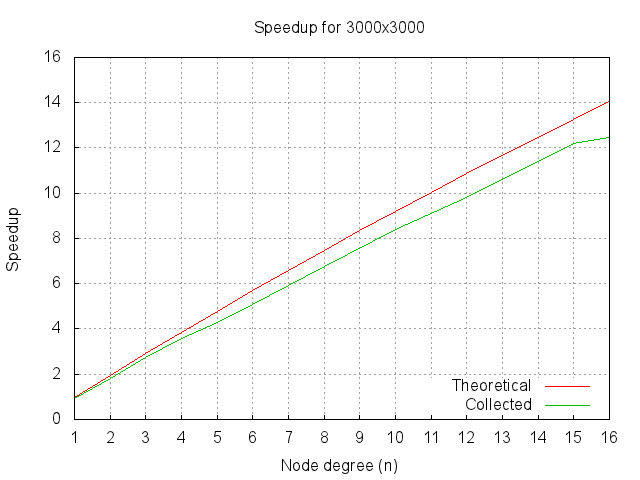
\includegraphics[width=0.45\textwidth]{plots/linsolve/speed-3000.png}
  }
  \subfigure{
    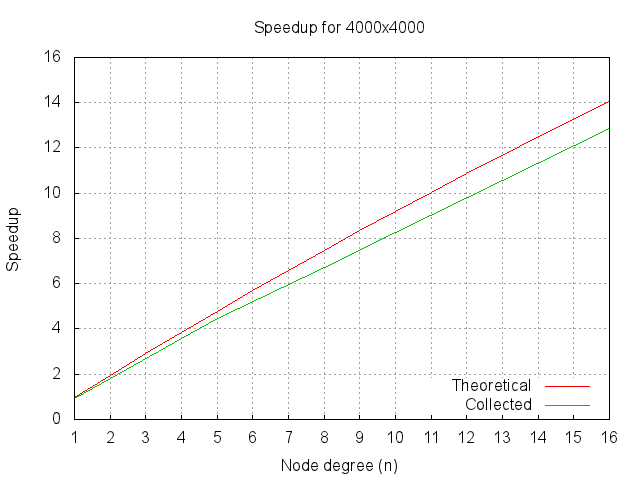
\includegraphics[width=0.45\textwidth]{plots/linsolve/speed-4000.png}
  }\\
  \subfigure{
    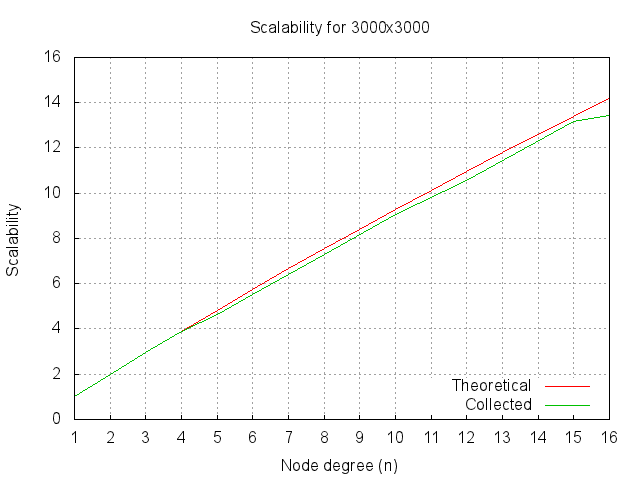
\includegraphics[width=0.45\textwidth]{plots/linsolve/scal-3000.png}
  }
  \subfigure{
    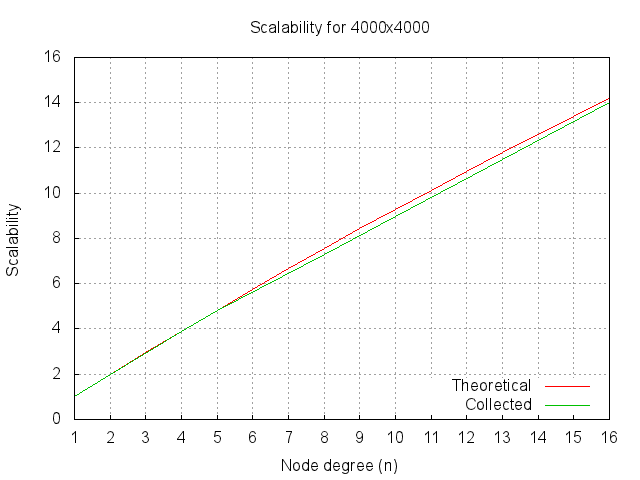
\includegraphics[width=0.45\textwidth]{plots/linsolve/scal-4000.png}
  }
  \caption{\texttt{linsolve} function: Efficiency, Speedup and Scalability}
  \label{fig:linsolve-scal-eff}
\end{figure}

This factor was further investigated and studied, by taking the standard
deviation on the registered time interval taken by each worker to
compute the given partition thus revealing some kind of asymmetry
between the \texttt{min} and \texttt{linsolve} functions. As reference
take in consideration Table~\ref{tbl:std-deviation}. From a rapid look
you can notice a magnitude of order of difference between the two
functions. This means that the $T_f$ parameter we take as reference
is not fixed but may vary depending on the input values and should have
taken as an average case measure. By the way, although slightly imprecise,
the curve still describe with a given approximation the real situation.

\begin{table}
  \centering
  \begin{tabular}{|r|r|r|}
    \hline
    \textbf{Inputs} & \texttt{min} & \texttt{linsolve} \\
    \hline
    3000            & 0.2143       & 1.296 \\
    \hline
    4000            & 0.1156       & 1.101 \\
    \hline
  \end{tabular}
  \caption{Average of standard deviation between workers calculation
  time}
  \label{tbl:std-deviation}
\end{table}

\section{Concrete implementation}\label{sec:concrete-impl}

Regarding the concrete implementation part, we decided to use
Python\footnote{\url{http://python.org}} programming language jointly
with \texttt{mpi4py}\footnote{\url{http://mpy4py.scipy.org}} library
which provides a wrapper to Message Passing Interface API specification.

Since Python (actually CPython the official Python implementation) does
not provide an efficient implementation of threads due to
GIL\footnote{\url{http://wiki.python.org/moin/GlobalInterpreterLock}}
(Global Interpreter Lock) we decided to just use process as method for
exploiting cluster of multi-cores resources. Regarding communications
everything is delegated to the library which is in charge of introducing
optimization whenever two workers are allocated on the same machine and
they need to exchange data.

We will start our analysis by taking a look to the \texttt{run.py}
(Listing~\ref{lst:run}) which is responsible to set up everything and
start the real computation. It accepts as parameter two parameters. The
first one may be set to ``seq'' to spawn the sequential version of the
program or to ``par'' for the parallel version. The second parameter
instead just pass the matrix file where the function should be applied
to. The program accepts an optional third parameter which gives
indication about the partition scheme. If it is not present the software
will try do some calculation to derive an optimal partition scheme by
following the procedure we have described in the
``\nameref{sec:abstract-impl}'' section.

As you can see in case of parallel version is required to be run, the
run function is called which is in charge of setting up the master
(\texttt{main} function) and the workers (\texttt{slave} function).

\lstinputlisting[label=lst:run,caption=Spawner: \texttt{run.py}]{../src/run.py}

The worker logic is presented in Listing~\ref{lst:slave}. The worker
just waits to receive its partition and then create a
\texttt{StencilWorker} instance and starts the computation.

\lstinputlisting[label=lst:slave,caption=Worker logic: \texttt{slave.py}]{../src/slave.py}

Listing~\ref{lst:main} shows the two function which are called by the
\texttt{run.py} module. The first function is the one responsible for
the parallel execution of the program, while the second is meant for
sequential execution. Instrumentation code is also present to take into
account loading time of the matrix, and completion time.

\lstinputlisting[label=lst:main,caption=Master logic: \texttt{main.py}]{../src/main.py}

Now we will go deeper in the analysis of the stencil skeleton by
introducing Listing~\ref{lst:stencil}. The main class in this case is
the \texttt{Stencil} whose constructor takes as parameter the input
offset set. Immediately after the \texttt{analyze\_offsets} method is
called which is in charge of extracting communication data dependencies
and to convert them into elementary vectors tuples. This is needed
whenever a dependency of the type \emph{($x$,$y$)} with $x \ne 0$ and $y
\ne 0$ is present. In this specific case all the input offsets are
analyzed to derive a tuple like \emph{($max_{x}, max_{y}$)}, for the
composed directions (\eg up-left, down-right, \ldots).

The \texttt{apply} function is the most important function in this
class. It is in charge of deriving a proper partition scheme in case (if
required, by calling the homonym method) and to scatter the matrix among
the workers. Method \texttt{fix\_data\_dep} is called before the actual
scattering phase takes place. This is necessary to avoid bogus
function evaluation in various corner cases, such the one depicted in
Figure~\ref{fig:corner}.

\begin{figure}[!h]
  \centering
  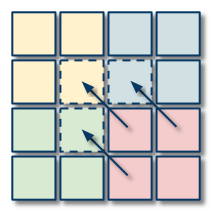
\includegraphics[width=0.2\textwidth]{imgs/corner.png}
  \caption{Bogus data derivation}
  \label{fig:corner}
\end{figure}

In this situation, a partition $2\times2$ is derived while the input
offset set is equal to \emph{(-1, -1)}. Therefore although not only the
up-left neighbor is involved but partially also the left and the upper
neighbors. This corner case is verified whenever the composed direction
tuple ($x$, $y$) is lesser than the partition dimension ($x < height
\lor y < width$). If this condition is met, \texttt{fix\_data\_dep}
function is in charge of adding redundant communication to the pattern
(in this case the communication with the up and left neighbors).

After this check a phase of set-up is made, to interconnect the workers
by the mean of \texttt{autoconnect} method, which is called twice first
to connect left-, right-, up- and down- neighbors each other and then
for the remaining up-right, up-left, down-right and down-left neighbors.

Then the real scattering phase is done and after the gathering procedure
followed by a reconstruction phase. A final barrier is then used to
synchronize all the remote entities and conclude the execution.

Regarding the class \texttt{StencilWorker} which is in charge of
modeling the behaviour of the workers, no further comment is needed. The
class first sends the contour part of the partition to the other
workers, then it waits to receive the parts which are sent by the
other neighbors. After reception the calculation phase is executed by
making use of the \texttt{Puzzle} class. The final step is taking part
in the global gathering phase were each worker sends back to the master
(node with rank 0) its own computed part.

\lstinputlisting[label=lst:stencil,caption=Stencil skeleton implementation: \texttt{stencil.py}]{../src/stencil.py}

Listing~\ref{lst:puzzle} presents the class which is used by the
\texttt{StencilWorker} to re-arrange all contour partitions received by
the neighbors in a new sub-matrix, which will then be used to execute
the evaluation of the functional code. We make use of utilities
functions such as \texttt{vstack} and \texttt{hstack} which are provided
by the \texttt{numpy}\footnote{\url{http://numpy.scipy.org}} library,
respectively to vertically or horizontally stack small matrices into
bigger ones.

\lstinputlisting[label=lst:puzzle,caption=Stencil skeleton implementation: \texttt{puzzle.py}]{../src/puzzle.py}

To finish our analysis we present the communicator class which is
responsible to exchange data between workers whenever there is the
necessity to do it. Listing~\ref{lst:mpi} presents the
\texttt{Communicator} class, which provides communication by means of
MPI API specification. The only method which deserves an explanation is
the \texttt{send} method. It is in charge, by looking in the
\texttt{data\_segment} structure, to literary extract the needed
sub-matrix from the central one. This is done by the means of the
\texttt{extract} method provided by the high-level \texttt{Matrix}
class.

\lstinputlisting[label=lst:mpi,caption=Communication: \texttt{communicator/mpi.py}]{../src/communicator/mpi.py}

Listing~\ref{lst:enum} is presented just to complete the global vision.
It just contains various constants and enumerations which are used in
various part of the code, and the \texttt{Connections} class which is
just a class placeholder that is used to store information about the
connections between workers (neighbor information).

\lstinputlisting[label=lst:enum,caption=Communication constants: \texttt{communicator/enum.py}]{../src/communicator/enum.py}


The last file is the higher level encapsulation of the
\texttt{numpy.array} data structure. The class \texttt{Matrix} is shown
in Listing~\ref{lst:matrix}. Besides typical methods, such as
\texttt{get set} or \texttt{random}, it provides also a
\texttt{derive\_partition} method which applies the same reasoning we
have presented in Section~\ref{sec:abstract-impl} to derive an optimal
partitioning scheme and \texttt{extract} which is used by the
\texttt{Puzzle} class as mentioned before.

\lstinputlisting[label=lst:matrix,caption=Matrix class: \texttt{matrix.py}]{../src/matrix.py}

Regarding the functional code this is simply stored in the
\texttt{functional.py} file presented in Listing~\ref{lst:functional}.
In the file the \texttt{offsets} variable and a function named
\texttt{function} is exported to the other modules.

\lstinputlisting[label=lst:functional,caption=Functional code: \texttt{functional.py}]{../src/functional.py}

\section{Build instructions}

In order to successfully run the source code you need at least CPython
2.5.x. For getting a usable build of \texttt{mpi4py} package you need a
compiler and the development file of the CPython. You can easily
install them by typing:

\begin{verbatim}
$ apt-get install python python-dev gcc
\end{verbatim}

To avoid installing the extension system wide, we have used
\texttt{virtualenv}\footnote{\url{http://pypi.python.org/pypi/virtualenv}}
to create an isolated Python environment.

\begin{verbatim}
$ wget http://pypi.python.org/packages/source/v/virtualenv/virtualenv-1.6.1.tar.gz
$ tar xfz virtualenv-1.6.1.tar.gz
$ python virtualenv-1.6.1/virtualenv.py mpi
New python executable in mpi/bin/python
Installing setuptools............done.
Installing pip...............done.
$ . mpi/bin/activate
(mpi) $
\end{verbatim}

After creating the environment you can install the MPI python wrapper.
In our test-bed we were using machines with
\texttt{MPICH-1}\footnote{\url{http://www.mcs.anl.gov/research/projects/mpich2/}}
implementation of the 1.0 MPI API specification.

In our case since MPIv1.0 is not well supported we have to do some
tricks in order to get a working build. We have to thank Lisandro Dalcin
the author of the library for his precious support.

\begin{verbatim}
(mpi) $ http://mpi4py.googlecode.com/files/mpi4py-1.2.2.tar.gz
(mpi) $ tar xfz mpi4py-1.2.2.tar.gz && cd mpi4py-1.2.2

# This is needed to fix bogus error message in the finalization state.
# Take a look to http://code.google.com/p/mpi4py/issues/detail?id=20 for
# more information
(mpi) $ wget http://mpi4py.googlecode.com/svn/trunk/src/python.c -O src/python.c
(mpi) $ export MPICC=/usr/bin/mpicc.mpich
(mpi) $ export MPICH_USE_SHLIB=yes
(mpi) $ python setup.py install
(mpi) $ python setup.py build_exe
(mpi) $ python setup.py install_exe
\end{verbatim}

At the end of this phase you should have a \texttt{python2.5-mpi}
executable installed under \texttt{mpi/bin/} directory. Now to run a
specific test you have first to create a random matrix. You have to
change the current directory and make it point to
\texttt{skippy/src}. Then simply spawn a python interpreter and type:

\begin{minted}{pycon}
Python 2.5.2 (r252:60911, Jan  4 2009, 17:40:26) 
[GCC 4.3.2] on linux2
Type "help", "copyright", "credits" or "license" for more information.
>>> import matrix
>>> import cPickle # For serialization
>>> cPickle.dump(matrix.Matrix.random(3000, 3000), open("/tmp/matrix-3000-3000.mtx", "w"))
>>> quit()
\end{minted}

This should create a randomly filled matrix 3000 by 3000 in your
\texttt{/tmp} directory. Now to run the program on different machines
you have to write down a \emph{machinefile} which contains the
specification about the machines to use in your network. For our tests
we have used the following file:

\begin{verbatim}
axth1.cli.di.unipi.it:3
axth3.cli.di.unipi.it:2
axth4.cli.di.unipi.it:2
axth6.cli.di.unipi.it:2
axth7.cli.di.unipi.it:2
axth8.cli.di.unipi.it:2
axth10.cli.di.unipi.it:2
axth15.cli.di.unipi.it:2
axth29.cli.di.unipi.it:2
axth34.cli.di.unipi.it:2
\end{verbatim}

The syntax is pretty straightforward, first the machine host-name or IP
address, followed by colon and then by the number of slots to reserve on
that specific machine. Than to run the test you can simply type:

\begin{verbatim}
(mpi) $ mpirun -machinefile multicores -np 3 `pwd`/mpi/bin/python2.5-mpi \
        run.py par /tmp/matrix-3000-3000.mtx 3000x1500
3.8472688198 seconds to load the matrix
INFO:stencil:Skipping auto-derivation
INFO:stencil:After partition => Rows: 1 Cols: 2
INFO:stencil:Worker started on processor 1 axth15.cli.di.unipi.it
INFO:stencil:3.3783619404 seconds to scatter the matrix
INFO:stencil:Worker started on processor 2 axth27.cli.di.unipi.it
INFO:puzzle:0.0981070995 seconds to create auxiliary matrix
INFO:puzzle:0.1032311916 seconds to create auxiliary matrix
INFO:stencil:Worker 0: 27.8885238171 seconds to compute the partition
INFO:stencil:Sending back the computed sub-partition from 1
INFO:stencil:Worker 1: 29.1980512142 seconds to compute the partition
INFO:stencil:Sending back the computed sub-partition from 2
INFO:stencil:Worker 0: 2.8959200382 seconds to send back the partition
INFO:stencil:Worker 1: 3.1485359669 seconds to send back the partition
INFO:stencil:32.5039210320 seconds to gather the results
INFO:stencil:0.1175770760 seconds to reconstruct the result
INFO:stencil:Terminated.
36.0049271584 seconds to apply on 2 processors
\end{verbatim}
